\documentclass[c]{beamer}  % [t], [c], или [b] --- вертикальное выравнивание на слайдах (верх, центр, низ)

%\documentclass[handout]{beamer} % Раздаточный материал (на слайдах всё сразу)
%\documentclass[aspectratio=169]{beamer} % Соотношение сторон

%\usetheme{Berkeley} % Тема оформления
%\usetheme{Bergen}
%\usetheme{Szeged}

%\usecolortheme{beaver} % Цветовая схема
%\useinnertheme{circles}
%\useinnertheme{rectangles}

%%% Работа с русским языком
\usepackage{cmap}					% поиск в PDF
\usepackage{mathtext} 				% русские буквы в формулах
\usepackage[T2A]{fontenc}			% кодировка
\usepackage[utf8]{inputenc}			% кодировка исходного текста
\usepackage[english,russian]{babel}	% локализация и переносы

%% Beamer по-русски
\newtheorem{rtheorem}{Теорема}
\newtheorem{rproof}{Доказательство}
\newtheorem{rexample}{Пример}

%%% Дополнительная работа с математикой
\usepackage{amsmath,amsfonts,amssymb,amsthm,mathtools} % AMS
\usepackage{icomma} % "Умная" запятая: $0,2$ --- число, $0, 2$ --- перечисление

%% Номера формул
\mathtoolsset{showonlyrefs=true} % Показывать номера только у тех формул, на которые есть \eqref{} в тексте.
%\usepackage{leqno} % Нумерация формул слева

%% Свои команды
\DeclareMathOperator{\sgn}{\mathop{sgn}}

%% Перенос знаков в формулах (по Львовскому)
\newcommand*{\hm}[1]{#1\nobreak\discretionary{}
{\hbox{$\mathsurround=0pt #1$}}{}}

%%% Работа с картинками
\usepackage{graphicx}  % Для вставки рисунков
\graphicspath{{images/}{images2/}}  % папки с картинками
\setlength\fboxsep{3pt} % Отступ рамки \fbox{} от рисунка
\setlength\fboxrule{1pt} % Толщина линий рамки \fbox{}
\usepackage{wrapfig} % Обтекание рисунков текстом

%%% Работа с таблицами
\usepackage{array,tabularx,tabulary,booktabs} % Дополнительная работа с таблицами
\usepackage{longtable}  % Длинные таблицы
\usepackage{multirow} % Слияние строк в таблице

%%% Программирование
\usepackage{etoolbox} % логические операторы

%%% Другие пакеты
\usepackage{lastpage} % Узнать, сколько всего страниц в документе.
\usepackage{soul} % Модификаторы начертания
\usepackage{csquotes} % Еще инструменты для ссылок
%\usepackage[style=authoryear,maxcitenames=2,backend=biber,sorting=nty]{biblatex}
\usepackage{multicol} % Несколько колонок

%%% Картинки
\usepackage{tikz} % Работа с графикой
\usepackage{pgfplots}
\usepackage{pgfplotstable}

\begin{document}
    
\begin{frame}
    \centering{\textbf{{\Large Brain Tennis}}}
    
    \vspace{2ex}
    \centering{\small \textit{ИПММ-186}}
    
    \vspace{2ex}
    \url{https://github.com/winter-yuki/neuro-game} 
\end{frame} % Название проекта
\documentclass[a4paper,12pt]{article}

% В этом документе преамбула

%%% Работа с русским языком
\usepackage{cmap}					% поиск в PDF
\usepackage{mathtext} 				% русские буквы в формулах
\usepackage[T2A]{fontenc}			% кодировка
\usepackage[utf8]{inputenc}			% кодировка исходного текста
\usepackage[english,russian]{babel}	% локализация и переносы
\usepackage{indentfirst}
\frenchspacing

\renewcommand{\epsilon}{\ensuremath{\varepsilon}}
\renewcommand{\phi}{\ensuremath{\varphi}}
\renewcommand{\kappa}{\ensuremath{\varkappa}}
\renewcommand{\le}{\ensuremath{\leqslant}}
\renewcommand{\leq}{\ensuremath{\leqslant}}
\renewcommand{\ge}{\ensuremath{\geqslant}}
\renewcommand{\geq}{\ensuremath{\geqslant}}
\renewcommand{\emptyset}{\varnothing}
\newcommand*{\ooline}[1]{\overline{\overline{#1}}}
\newcommand*{\defe}{\overset{\underset{\mathrm{def}}{}}{=}}

%%% Дополнительная работа с математикой
\usepackage{amsmath,amsfonts,amssymb,amsthm,mathtools} % AMS
\usepackage{icomma} % "Умная" запятая: $0,2$ --- число, $0, 2$ --- перечисление

%% Номера формул
\mathtoolsset{showonlyrefs=true} % Показывать номера только у тех формул, на которые есть \eqref{} в тексте.
%\usepackage{leqno} % Нумереация формул слева

%% Свои команды
\DeclareMathOperator{\sgn}{\mathop{sgn}}

%% Перенос знаков в формулах (по Львовскому)
\newcommand*{\hm}[1]{#1\nobreak\discretionary{}
{\hbox{$\mathsurround=0pt #1$}}{}}

%%% Работа с картинками
\usepackage{graphicx}  % Для вставки рисунков
\graphicspath{{images/}{images2/}}  % папки с картинками
\setlength\fboxsep{3pt} % Отступ рамки \fbox{} от рисунка
\setlength\fboxrule{1pt} % Толщина линий рамки \fbox{}
\usepackage{wrapfig} % Обтекание рисунков текстом

%%% Работа с таблицами
\usepackage{array,tabularx,tabulary,booktabs} % Дополнительная работа с таблицами
\usepackage{longtable}  % Длинные таблицы
\usepackage{multirow} % Слияние строк в таблице

%%% Теоремы
\theoremstyle{plain} % Это стиль по умолчанию, его можно не переопределять.
\newtheorem{theoremm}{Теорема}[section]
\newtheorem{propositionn}[theoremm]{Утверждение}
\newtheorem{algorithmm}[theoremm]{Алгоритм}
\newenvironment{theorem}[1][Теорема]{%
    \begin{theoremm}[#1]$ $\par\nobreak\ignorespaces
    }{%
    \end{theoremm}
}
\newenvironment{proposition}[1][Утверждение]{%
    \begin{propositionn}[#1]$ $\par\nobreak\ignorespaces
    }{%
    \end{propositionn}
}
\newenvironment{algorithm}[1][Алгоритм]{%
    \begin{algorithmm}[#1]$ $\par\nobreak\ignorespaces
    }{%
    \end{algorithmm}
}

\theoremstyle{definition} % "Определение"
\newtheorem{corollary}{Следствие}[theoremm]
\newtheorem{problem}{Задача}[section]

\theoremstyle{remark} % "Примечание"
\newtheorem*{nonum}{Решение}

%%% Программирование
\usepackage{etoolbox} % логические операторы
\usepackage{listings} 

%%% Страница
\usepackage{extsizes} % Возможность сделать 14-й шрифт
\usepackage{geometry} % Простой способ задавать поля
	\geometry{top=35mm}
	\geometry{bottom=35mm}
	\geometry{left=10mm}
	\geometry{right=10mm}
 %
%\usepackage{fancyhdr} % Колонтитулы
% 	\pagestyle{fancy}
 	%\renewcommand{\headrulewidth}{0pt}  % Толщина линейки, отчеркивающей верхний колонтитул
% 	\lfoot{Нижний левый}
% 	\rfoot{Нижний правый}
% 	\rhead{Верхний правый}
% 	\chead{Верхний в центре}
% 	\lhead{Верхний левый}
%	\cfoot{Нижний в центре} % По умолчанию здесь номер страницы

\usepackage{setspace} % Интерлиньяж
%\onehalfspacing % Интерлиньяж 1.5
%\doublespacing % Интерлиньяж 2
%\singlespacing % Интерлиньяж 1

\usepackage{lastpage} % Узнать, сколько всего страниц в документе.

\usepackage{soul} % Модификаторы начертания

\usepackage{hyperref}
\usepackage[usenames,dvipsnames,svgnames,table,rgb]{xcolor}
\hypersetup{				% Гиперссылки
    unicode=true,           % русские буквы в раздела PDF
    pdftitle={Заголовок},   % Заголовок
    pdfauthor={Автор},      % Автор
    pdfsubject={Тема},      % Тема
    pdfcreator={Создатель}, % Создатель
    pdfproducer={Производитель}, % Производитель
    pdfkeywords={keyword1} {key2} {key3}, % Ключевые слова
    colorlinks=true,       	% false: ссылки в рамках; true: цветные ссылки
    linkcolor=red,          % внутренние ссылки
    citecolor=black,        % на библиографию
    filecolor=magenta,      % на файлы
    urlcolor=cyan           % на URL
}

\usepackage{csquotes} % Еще инструменты для ссылок

%\usepackage[style=authoryear,maxcitenames=2,backend=biber,sorting=nty]{biblatex}

\usepackage{multicol} % Несколько колонок

\usepackage{tikz} % Работа с графикой
\usepackage{pgfplots}
\usepackage{pgfplotstable}



\begin{document}

\textbf{Название проекта: }

\vspace{5ex}

\centering{\textbf{Ключевые роли в проекте}}

\begin{tabular}{|l|l|l|}
    \hline
    \textbf{Роль} & \textbf{ФИО} & \textbf{Контактная информация} \\
    \hline 
    Заказчик & Коваленко Геннадий & kovalenko@i-brain.tech \\
    %\hline
    %Спонсор проекта & Коваленко Генадий & kovalenko@i-brain.tech \\
    \hline
    Руководитель проекта & Стоян Андрей Сергеевич 
       & stoyan.yukio@gmail.com \\ 
     & & 8-904-333-89-81 \\ 
    \hline
    Команда проекта 
     & Костина Надежда Хасановна & nadianhasan@gmail.com \\ \cline{2-3}
     & Приймак Евгений Дмитриевич & eugenepriymak@yandex.ru \\ \cline{2-3}
     & Василевский Елисей Александрович & nexus\_s9@mail.ru \\ \cline{2-3}
     & Смиренский Павел Романович & clacter@bk.ru \\ \cline{2-3}
     & Счастливцев Никита Александрович & nikita-s4astlivtsev2012@yandex.ru \\ \cline{2-3}
     & Темиргалиев Рафаэль Анварович & rafantem@mail.ru \\
     & & 8-981-788-29-01 \\ \cline{2-3}
     & Дубровин Анатолий Максимович & dubrovinanatolii@mail.ru \\ 
     & & 8-965-766-05-07 \\
    \hline
\end{tabular}

\end{document} % конец документа

 % Команда проекта
\section{Постановка задачи}

\begin{frame}
\frametitle{\insertsection} 
Разработать соревновательное десктоп (ноут) приложение – многопользовательскую сетевую игру на базе интерфейса «мозг-компьютер», управляемую мысленными командами (воображением движений вместо реальных движений). Игрок - человек с нарушенными движениями (например, после инсульта и травм мозга).
\end{frame} % Первоначальная постановка задачи
\section{Цели проекта}

\begin{frame}
    \frametitle{\insertsection} 
    \framesubtitle{\insertsubsection}
    
    \begin{minipage}[h]{0.4\linewidth}
        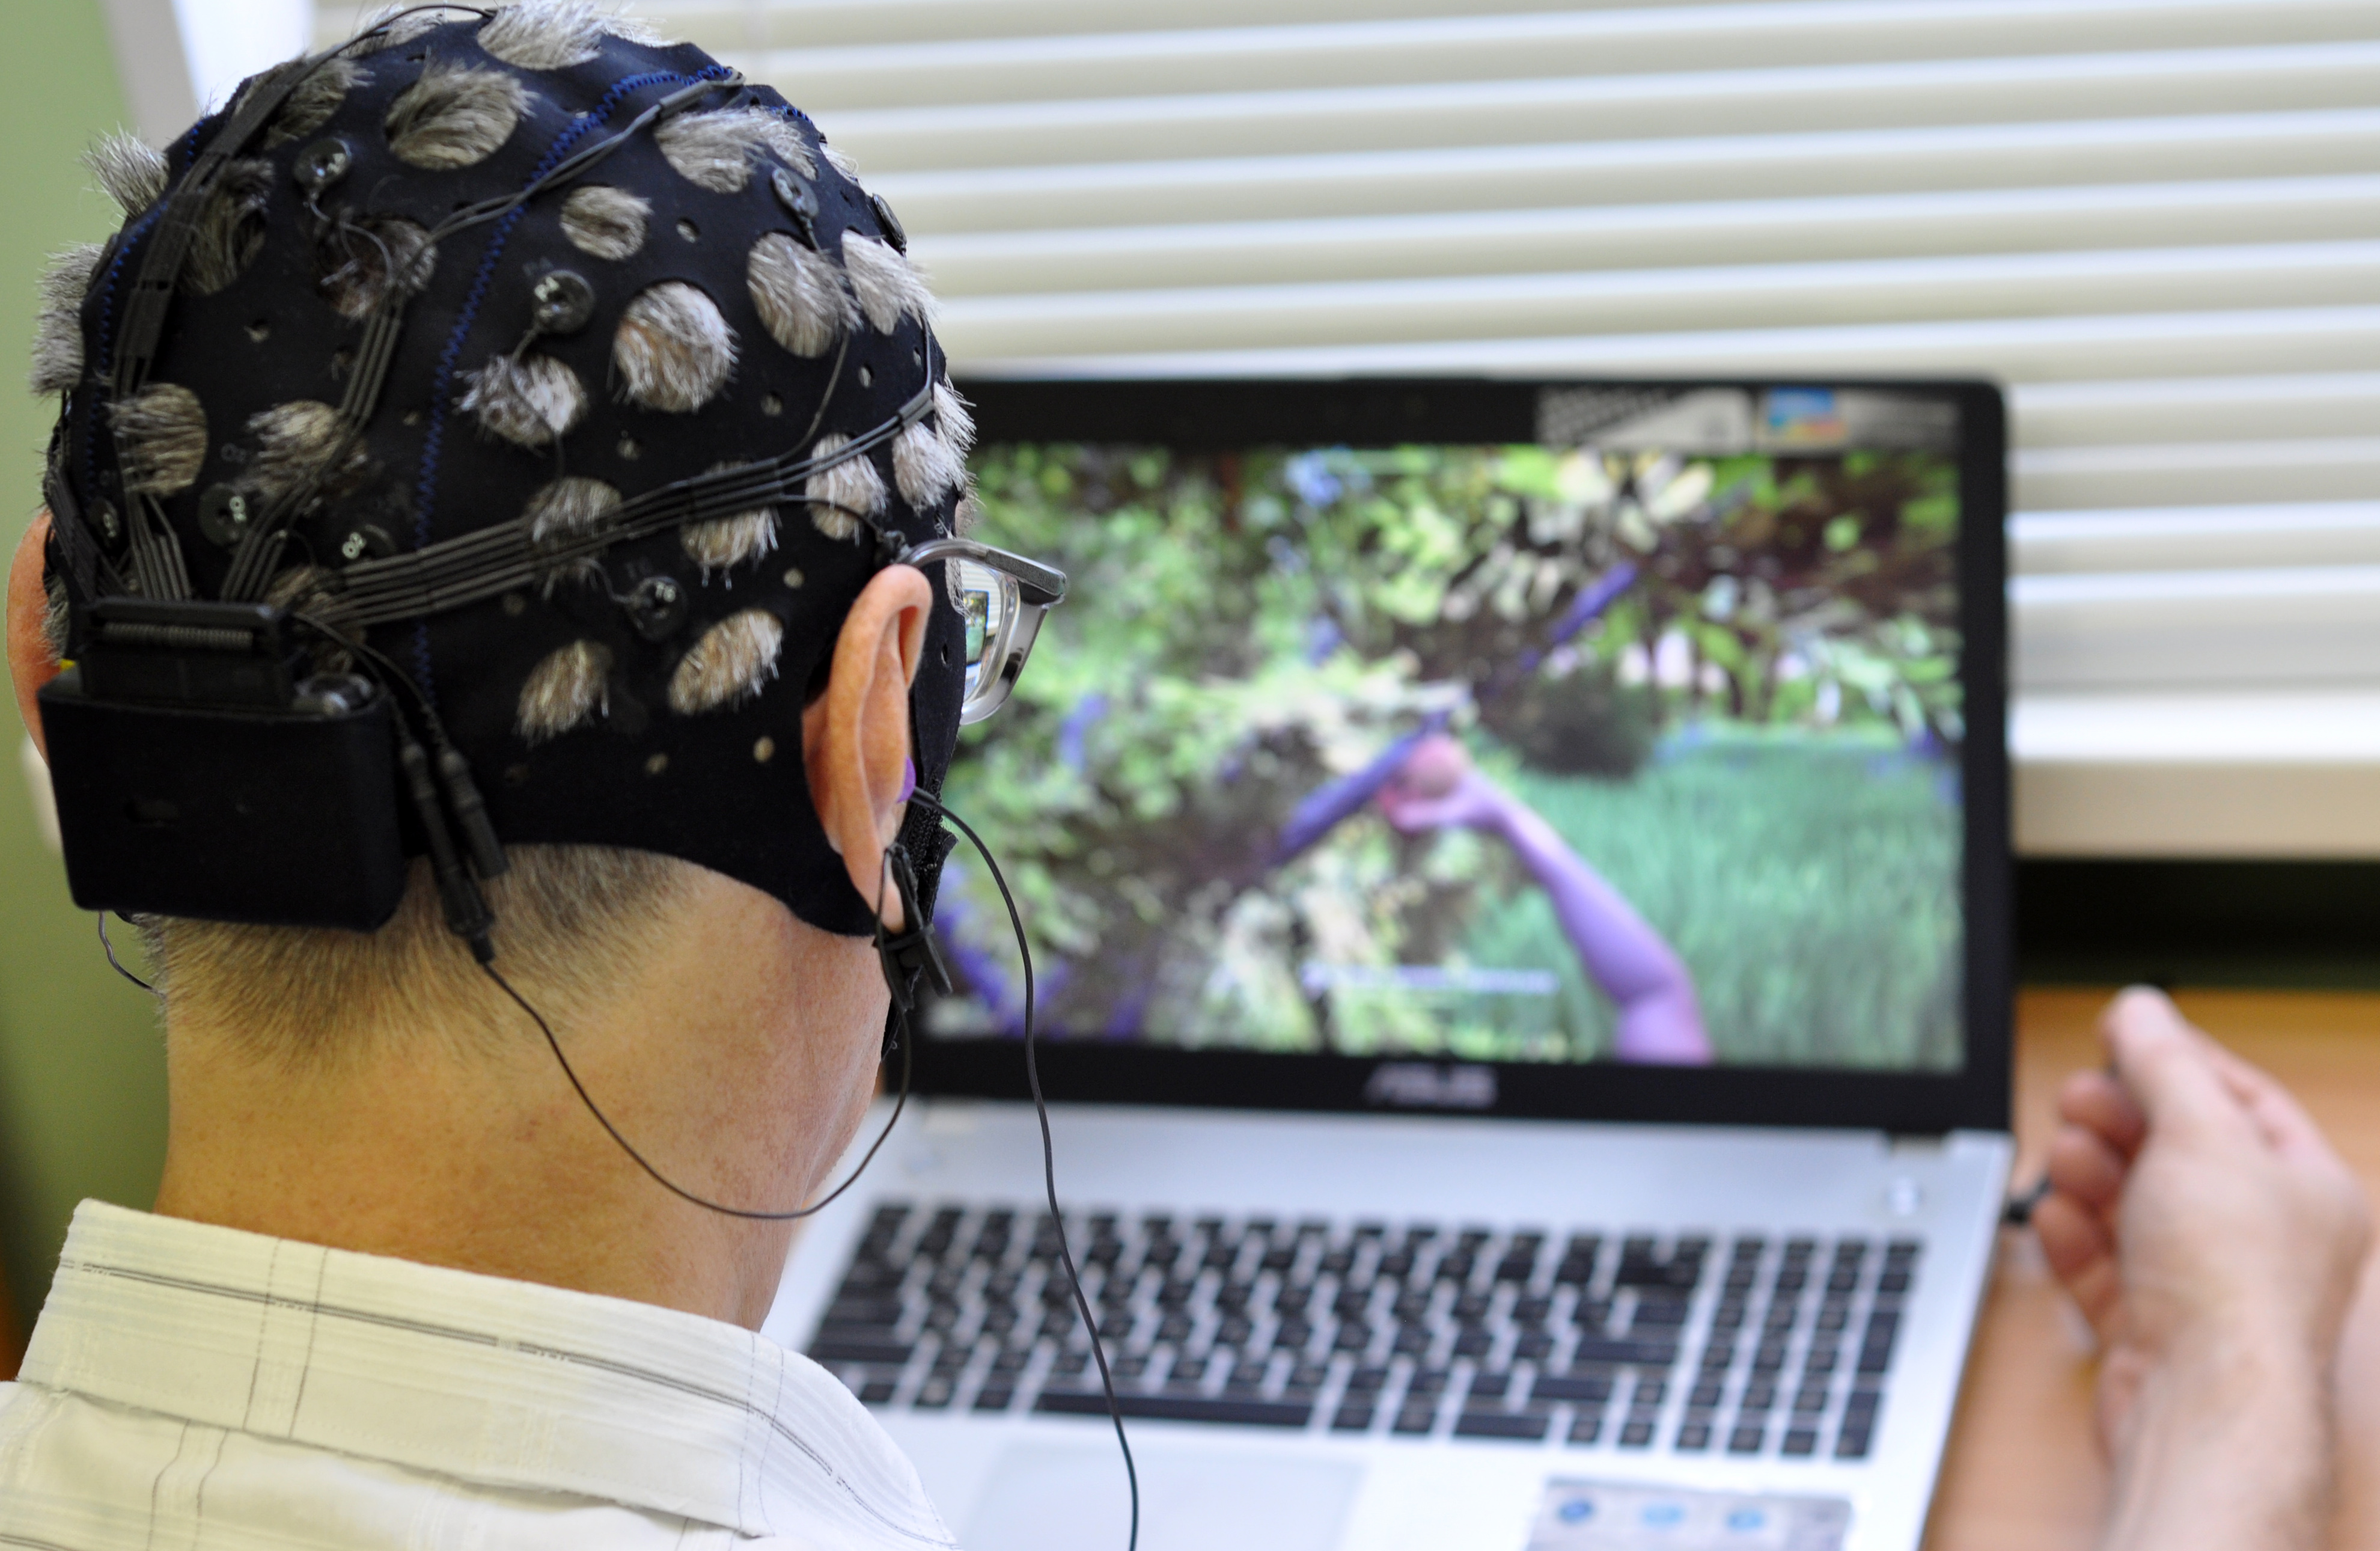
\includegraphics[width=\linewidth]{5.jpg}
    \end{minipage}
    \hfill 
    \begin{minipage}[h]{0.5\linewidth}
    \begin{itemize}
        \item Создание увлекательной игры.
        \item Увеличение эффективности реабилитационных процедур.
        \item Повысить стремление больных к выздоровлению.
    \end{itemize}
    \end{minipage}

\end{frame} % Цель проекта
\section{План выполнения проекта}

\begin{frame}
    \frametitle{\insertsection} 
    \begin{tabular}{|l|l|}
        \hline
        15 марта 2019 & проработка плана проекта \\
        \hline
        1 апреля 2019 &  исследование технологий \\
        \hline
        15 апреля 2019 & создание 3д сцены \\
        \hline
        1 мая 2019 & агрегация с ECS системой Qt \\
        \hline
        15 мая 2019 & геймплей \\
        \hline
        20 мая 2019 & доводка продукта и подготовка к презентации \\
        \hline
    \end{tabular}
\end{frame}
 % План выполнения проекта
\section{Выполненные этапы}

\begin{frame}
\frametitle{\insertsection} 
    \begin{itemize}
        \item разобрались в технологиях
        \item построили сцену
    \end{itemize}
\end{frame} % Выполненные этапы
\begin{frame}
    content
\end{frame} % Достигнутый результат
\begin{frame}
    content
\end{frame} % Проблемы
\section{Предлагаемое решение}

\begin{frame}
\frametitle{\insertsection} 
\framesubtitle{\insertsubsection}
\end{frame} % Предлагаемое решение
\section{Чем отличается от аналогов}

\begin{frame}
\frametitle{\insertsection} 

\begin{itemize}
    \item Гибкие настройки
    \item Сетевой режим
    %  TODO
\end{itemize}

\end{frame} % Чем отличается от аналогов
% Вопросы к заказчику


%\section{Актуальность}

\begin{frame}
\frametitle{\insertsection} 
\framesubtitle{\insertsubsection}
\end{frame}
%\section{Продукт проекта}

\begin{frame}
\frametitle{\insertsection} 
\framesubtitle{\insertsubsection}
Сетевая игра -- настольный теннис.
\end{frame}
%\section{Целевая аудитория}

\begin{frame}
\frametitle{\insertsection} 
\framesubtitle{\insertsubsection}

Люди, у которых из-за болезни ограничена способность к движению.

\end{frame}
%\section{Преимущества}

\begin{frame}
\frametitle{\insertsection} 
\framesubtitle{\insertsubsection}
    \begin{itemize}
        \item Высокий уровень кастомизации.
    \end{itemize}
\end{frame}
%\section{Сроки и бюджет}

\begin{frame}
\frametitle{\insertsection} 
\framesubtitle{\insertsubsection}
\begin{itemize}
    \item Сроки: 2 месяца
    \item Бюджет: 500р.
\end{itemize}
\end{frame}
%\section{Спасибо за внимание!}

\begin{frame}
\centering{\textbf{\Large Спасибо за внимание!}}
\end{frame}

\end{document}